The final continuous recording contains two transmissions at 120 cm and $\Delta\alpha=0.1$: first 2 bit/s, then 3 bit/s. The tone pairs were 4/8 Hz and 6/12 Hz, respectively. A fixed image-interior ROI was selected before decoding and used for both segments. Packet starts were estimated at 5.250 s and 43.775 s. The 38.525 s separation agrees with the original transmitter-log separation of 38.551 s to within one 30 fps camera frame. Both complete packets lie inside their assigned analysis windows.
\begin{table}[H]
\centering
\begin{tabular}{rrrrcc}
\hline
Raw rate & Duration & Correct-bit rate & Payload rate & BER & CRC \\
(bit/s) & (s) & (bit/s) & (bit/s) & & \\
\hline
2 & 26.500 & 2.00 & 0.906 & 0 & Pass \\
3 & 17.667 & 3.00 & 1.358 & 0 & Pass \\
\hline
\end{tabular}
\caption{Higher-rate results at 120 cm/$\Delta\alpha=0.1$. Each packet decoded as \texttt{CMU}, with 53 of 53 bits correct.}
\label{tab:fast}
\end{table}
\begin{figure}[H]
\centering
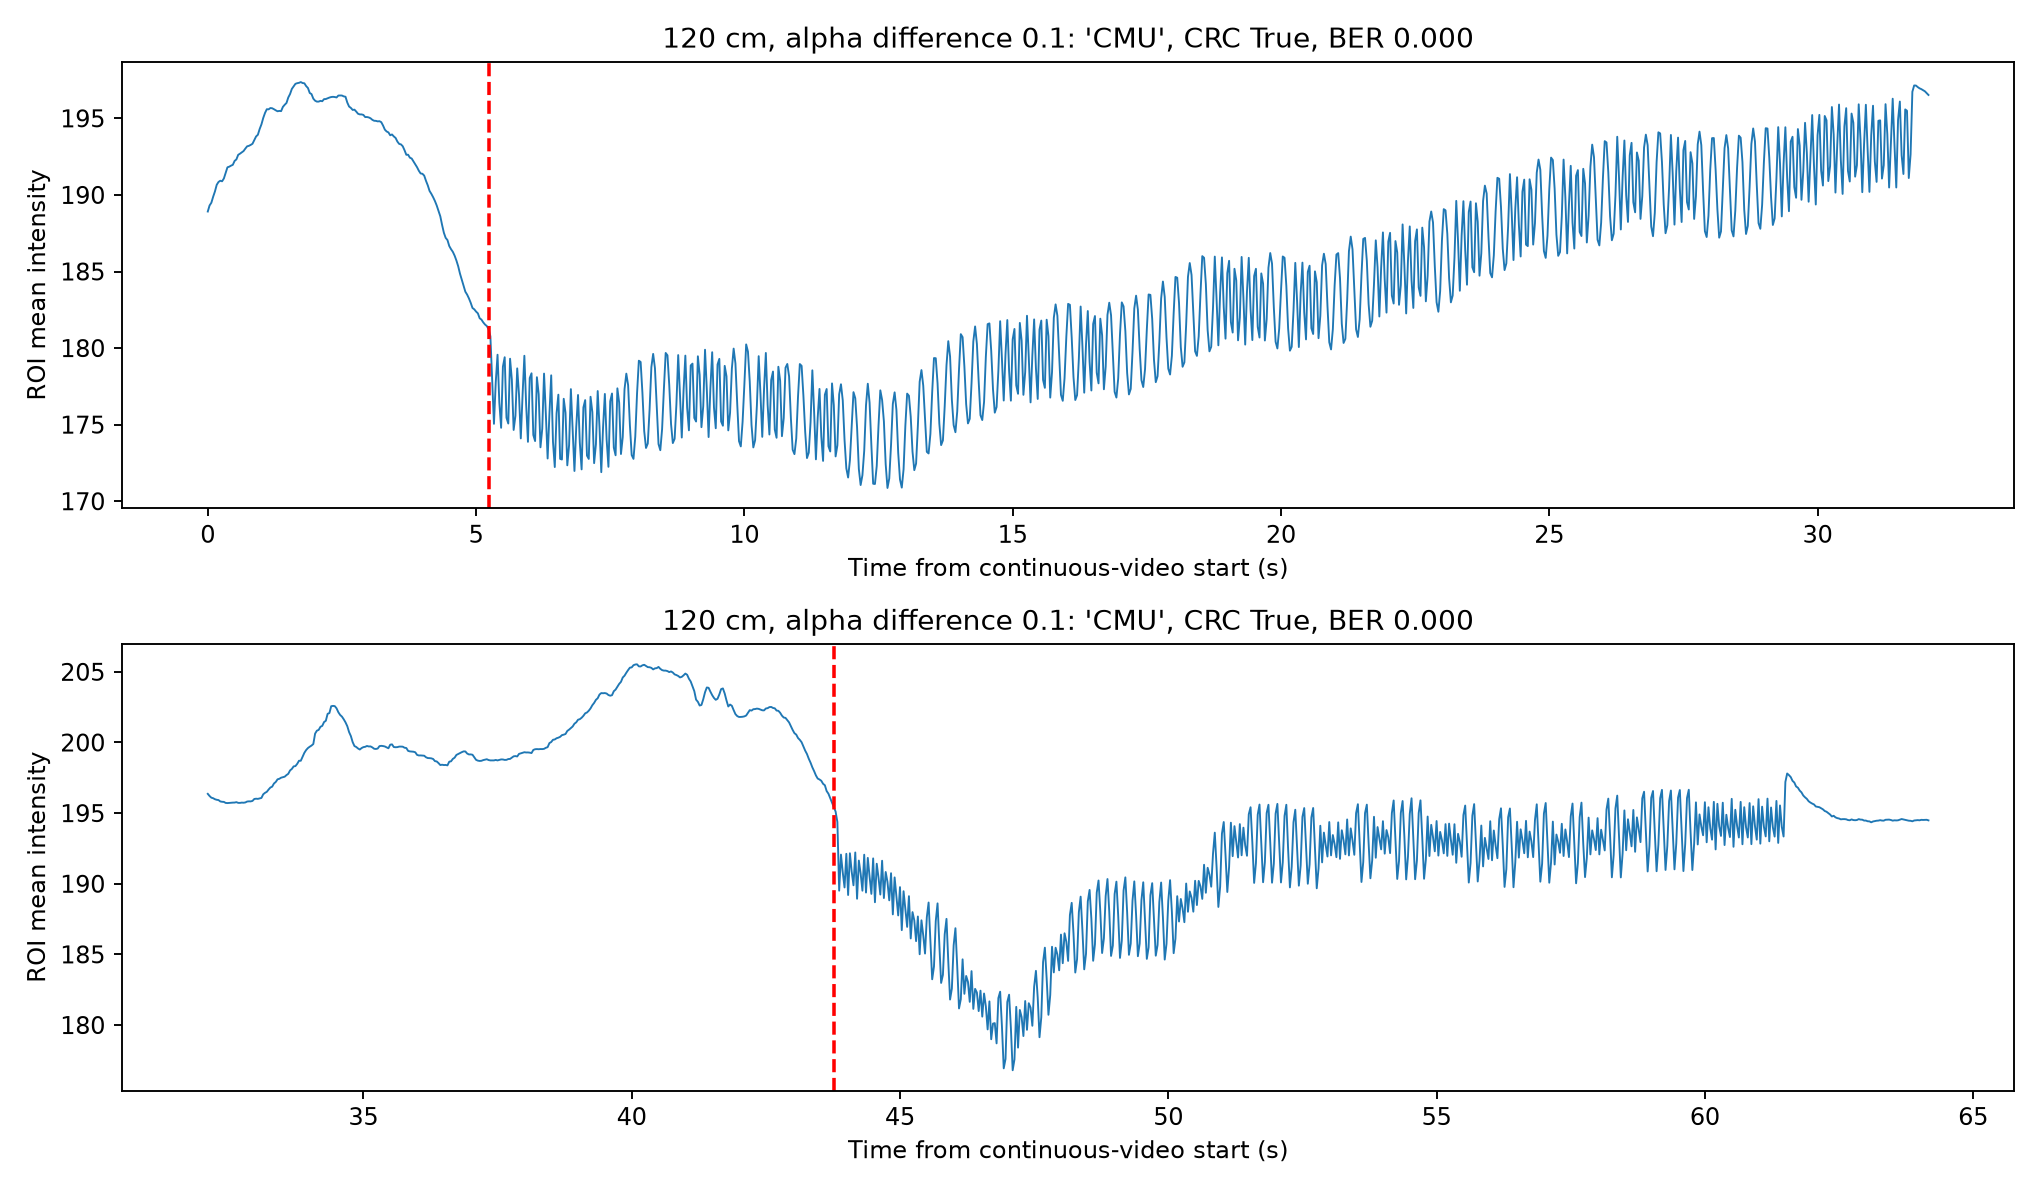
\includegraphics[width=\textwidth,height=6.7cm,keepaspectratio]{fast_transmissions.png}
\caption{The two higher-rate transmissions in the original continuous video. Dashed lines indicate packet starts selected using the public preamble.}
\label{fig:fast}
\end{figure}
The maximum successfully tested raw rate was 3 bit/s in this condition; this does not establish channel capacity or performance at untested combinations. At 30 camera frames/s, the 12 Hz tone has only about 2.5 samples per cycle, making exposure and frame timing relevant. The eight baseline packets and two faster packets contain 530 compared frame bits with no observed errors, subject to the qualified reference for the first baseline recording.

Both alpha differences were visibly flickering at the baseline rate. I also observed noticeable flicker in both the 2 and 3 bit/s recordings. Thus, imperceptible communication was not demonstrated within the tested rates, and a perceptual transition speed was not established.

An additional live phone demonstration is documented in the following subsection. It is reported separately from the 530-bit offline BER comparison above.
